% Emacs settings: -*-mode: latex; TeX-master: "manual.tex"; -*-

\chapter{Test results}
\label{testresults}

In this Appendix, we present a few illustrative
results from the three instruments presented in 
section \ref{s:instrument}. A more thorough presentation
may be found on the \MCS\ home page \cite{mcstas_webpage}.

\section{Scattering from the V-sample test instrument}
\label{s:vanadium-result}

In figure \ref{f:V-results}, we present the radial distribution 
of the scatting from an evenly illuminated V-sample,
as seen by a spherical PSD.
It is interesting to note that the variation in the
scattering intensity is as large as 10\%. This is an effect
of attenuation of the beam in the cylindrical sample.

\begin{figure}
  \begin{center}
    \includegraphics[width=0.6\textwidth]{figures/vanadium-surf-2.eps}
  \end{center}
\caption{Scattering from a V-sample, measured by a spherical
  PSD. The sphere has been transformed onto a plane and the intensity is
  plotted as the third dimension. A colour version of this picture is
  found on the title page of this manual.}
\label{f:V-results}
\end{figure}

\section{Simulated and measured resolution of TAS1}
\label{data:TAS1}

In order to test the \MCS\ package on a qualitative level,
we have performed a very detailed simulation of the conventional
triple axis spectrometer TAS1, Ris\o . The measurement series
constitutes a complete alignment of the spectrometer,
using the direct beam and scattering from V and Al$_2$O$_3$
samples at an incoming energy of 20.0~meV, using the second order
scattering from the monochromator. 
In the instrument definitions, we have used all available
information about the spectrometer. However, the
mosaicities of the monochromator and analyser are set
to 45' in stead of the quoted 30', since we from our
analysis believe this to be much closer to the truth.

In these simulations, we have tried to reproduce
every alignment scan with respect to position and width
of the peaks, whereas we have not tried to compare
absolute intensities. Below, we show a few comparisons 
of the simulations and the measurements. 

Figure \ref{f:2t_direct} shows a scan of 
$2\theta_s$ on the collimated direct beam in two-axis mode.
A 1 mm slit is placed on the sample position.
Both the measured width and non-Gaussian peak shape
are well reproduced by the \MCS\ simulations.

\begin{figure}
  \begin{center}
    \includegraphics[width=0.6\textwidth]{figures/tas1-2T.eps}
  \end{center}
\caption{Scans of $2\theta_s$ in the direct beam with 1 mm slit on the
  sample position.
"$\times$": measurements, "o": simulations  
Collimations: open-30'-open-open.}
\label{f:2t_direct}
\end{figure}

In contrast, a simulated $2\theta_a$ scan in triple-axis 
mode on a V-sample showed a surprising offset from zero, see
Figure \ref{f:v_2ta_offset}. However, a simulation with a PSD
on the sample position showed that the beam center was 1.5~mm
off from the center of the sample, and this was important
since the beam was no wider than the sample itself.
A subsequent centering of the beam resulted in a nice
agreement between simulation and measurements. 
For a comparison on a slightly different instrument
(analyser-detector collimator inserted), 
see Figure~\ref{f:v_2ta_zero}.

\begin{figure}
  \begin{center}
    \includegraphics[width=0.6\textwidth]{figures/vanadium-plot-1.eps}
  \end{center}
\caption{First simulated $2\theta_a$ scan on a vanadium sample.
Collimations: open-30'-28'-open.}
\label{f:v_2ta_offset}
\end{figure}

\begin{figure}
  \begin{center}
    \includegraphics[width=0.6\textwidth]{figures/vanadium-plot-2.eps}
  \end{center}
\caption{Corrected $2\theta_a$ scan on a V-sample.
Collimations: open-30'-28'-67'.
"$\times$": measurements, "o": simulations.}
\label{f:v_2ta_zero}
\end{figure}

The result of a $2\theta_s$ scan on an Al$_2$O$_3$
powder sample in two-axis mode is shown in Figure \ref{f:al2o3}.
Both for the scan in focusing mode (+ $-$ +)
and for the one in defocusing mode (+ + +) (not shown),
the agreement between simulation and experiment is excellent.

\begin{figure}
  \begin{center}
    \includegraphics[width=0.6\textwidth]{figures/al2o3-focus.eps}
  \end{center}
\caption{$2\theta_s$ scans on Al$_2$O$_3$ in two-axis, focusing mode.
Collimations: open-30'-28'-67'.
"$\times$": measurements, "o": simulations.  
A constant background is added to the simulated data.}
\label{f:al2o3}
\end{figure}

As a final result, we present a scan of the energy
transfer $E_a = \hbar \omega$ on a V-sample.
The data are shown in Figure \ref{f:v_ea}.

\begin{figure}
  \begin{center}
    \includegraphics[width=0.6\textwidth]{figures/ea-scan.eps}
  \end{center}
\caption{Scans of the analyser energy on a V-sample.
Collimations: open-30'-28'-67'.
"$\times$": measurements, "o": simulations.}
\label{f:v_ea}
\end{figure}


\section{Simple spectra from the PRISMA instrument}
\label{data:PRISMA}

A plot from the detector in the PRISMA simulation is shown in Figure
\ref{f:PRISMAdata}. These results were obtained with each analyser blade
rotated one degree relative to the previous one. The separation of the
spectra of the different analyser blades is caused by different energy
of scattered neutrons and different flight path length from source to
detector.  We have not performed any quantitative analysis of the data at this
time.

\begin{figure}
  \begin{center}
    \includegraphics[width=0.6\textwidth]{figures/prisma2-a.eps}
  \end{center}
\caption{Test result from PRISMA instrument using ``coloured
  neutrons''. Each graph shows the neutrons scattered from one analyser blade.}
\label{f:PRISMAdata}
\end{figure}

